% common part for every lection

\documentclass{beamer}

\usetheme{Warsaw}
\usefonttheme[onlylarge]{structurebold}
\setbeamerfont*{frametitle}{size=\normalsize,series=\bfseries}
\setbeamertemplate{navigation symbols}{}

\usepackage{pdfpages}
\usepackage{soul}
\usepackage{ucs}
\usepackage[utf8x]{inputenc}
\usepackage[TS1,T2A]{fontenc}
\usepackage[english,russian]{babel}
\usepackage{times}
\usepackage{listings}

\author[Author, Vlad Shakhov]{Влад 'mend0za' Шахов\\Linux \& Embedded Team Leader}

\institute[SaM Solutions]
{
  Linux \& Embedded Department
}

\date[Dec 2012]

\subject{Linux QA training}

\pgfdeclareimage[height=1.5cm]{sam-solutions-logo}{clipart/sam-solutions-elinux}

\logo{\pgfuseimage{sam-solutions-logo}}

\graphicspath{{./clipart/}}



\title[SaM Solutions. Linux QA Training]
{
  Занятие 2.\\
  Bourne Shell aka POSIX sh.
}

\begin{document}
\begin{frame}
  \titlepage
\end{frame}

\section{Введение в Shell}

\begin{frame}
  \frametitle{Что такое Unix shell?}
  
  \alert{Что такое Unix shell? (Назойливый повтор)}

  \begin{itemize}
    \item Обычная программа, запускающаяся после входа в систему
    \item Интерактивный командный интерпретатор
    \item Язык программирования
    \item Платформа интеграции (для утилит)
    \item Сотни разных реализаций (bash, ksh, zsh, tcsh, \ldots )
    \item Масса различных диалектов
  \end{itemize}

\end{frame}

\begin{frame}[fragile]
  \frametitle{Shell. Ключевые понятия - 1}
  \framesubtitle{Определения}

  \begin{itemize}
    \item \alert{Приглашение командной строки (CMD PROMPT)}: \pause 
      \begin{verbatim}
	$, #, user@host:~$
      \end{verbatim} \pause
    \item \alert{Команда}: \newline \verb+whoami; top; exit+ \pause
    \item \alert{Параметр}: \newline \verb+man bash; who am i+ \pause
    \item \alert{Ключ (1 символ)}: \newline \verb+ls -a; ls -al; ls -a -l /tmp/+ \pause
    \item \alert{Длинный ключ (GNU-style}: \newline \verb+ls --version+
  \end{itemize}
\end{frame}

\begin{frame}
  \frametitle{Shell. Ключевые понятия - 2}
  \framesubtitle{Картинка для закрепления}
    \hbox{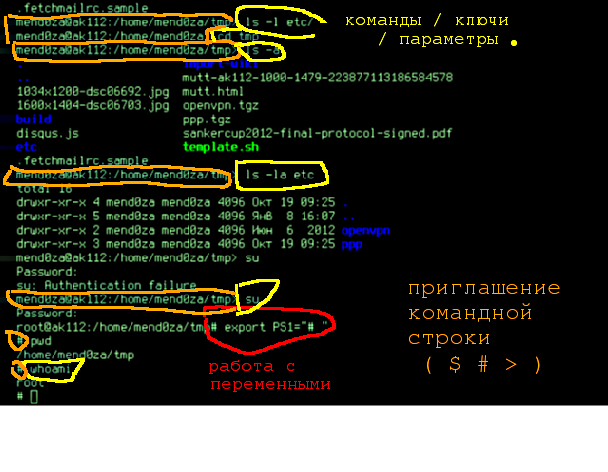
\includegraphics[height=7cm]{bash-input-screenshot}}
\end{frame}

\section{Интерактивная работа в Shell}

\begin{frame}
  \frametitle{Приёмы эффективной работы}

  \alert{\Large{Как в Shell работать быстро?}} 
  \pause

  \begin{enumerate}
    \item \Large{автодополнение путей и команд}
    \item \Large{история команд}
    \item \Large{редактирование командной строки}
  \end{enumerate}

\end{frame}

\begin{frame}[fragile]
  \frametitle{Приёмы эффективной работы}
  \framesubtitle{Автодополнение путей и команд - 1}

  \alert{\Large{Волшебная кнопка - TAB}} \newline
  \pause
  \begin{itemize}
    \item \Large{Имя команды} \pause \newline
      \small{Пример: \verb+mys[TAB]_co[TAB]+} \pause \newline
      \small{Результат: \verb+mysql_convert_table_format+} \newline
      \alert{8 vs 26} \pause
    \item \Large{Пути и имена файлов} \pause \newline
      \small{Пример: \verb+ls /u[TAB]lo[TAB]sh[TAB]/ca[TAB]+} \pause \newline
      \small{Результат: \verb+ls /usr/local/share/ca-certificates/+} \newline
      \alert{16 vs 36} \pause
    \item \Large{Параметры и ключи} \footnote{Только у BASH и ZSH (если настроены)} \pause \newline
      \small{Пример: \verb+apti[TAB]--a[TAB]sh[TAB]core[TAB][ENTER]+} \pause \newline
      \small{Результат: \verb+aptitude --assume-yes show coreutils+} \newline
      \alert{16 vs 37} \pause
  \end{itemize}
\end{frame}

\begin{frame}
  \frametitle{Приёмы эффективной работы}
  \framesubtitle{Автодополнение путей и команд - 2}
  
  \Large{\alert{Единственный вариант подстановки}: \newline TAB дополняет сразу} \pause

  \Large{\alert{Несколько вариантов подстановки?}} 

  \Large{Ещё больше волшебства - 2 кнопки TAB!} 

  \Large{\alert{2xTAB - список вариантов подстановки}}
\end{frame}

\begin{frame}[fragile]
  \frametitle{Приёмы эффективной работы}
  \framesubtitle{Автодополнение путей и команд - 3}
  
  \Huge{Примеры}

  \Large{
  \begin{itemize}
    \item apt[TAB][TAB]
    \item \verb+aptitude --[TAB][TAB]+\footnote{Только для BASH и ZSH}
    \item ls /[TAB][TAB] \footnote{Можно использовать вместо команды ``ls''}
  \end{itemize}
      }
\end{frame}
  

\begin{frame}
  \frametitle{Приёмы эффективной работы}
  \framesubtitle{История команд}

  \Large{\alert{Просмотр истории}}

  \begin{itemize}
    \item ``Up'' и ``Down'' - вперёд-назад \pause
    \item ``Ctrl+R'' - интерактивный поиск в истории \pause
    \item повторно ''Ctrl+R`` - искать дальше
  \end{itemize}
\end{frame}

\begin{frame}
  \frametitle{Приёмы эффективной работы}
  \framesubtitle{Редактирование командной строки}

  \Large{\alert{Emacs editing mode}} \footnote{Только KSH-совместимые: bash, zsh, pdksh, mksh, etc}

  \begin{itemize}
    \item ``Left'' и ``Right'' - вперёд-назад по текущей строке \pause
    \item ``Ctrl+a'' и ``Ctrl+e''  - перейти в начало и конец строки \pause
    \item ``Ctrl+u'' - удалить от курсора до начала строки \pause
    \item ``Ctrl+w'' - удалить слово (от курсора до разделителя, влево) 
  \end{itemize}
    
\end{frame}

\section{Язык shell}

\subsection{Код возврата}

\begin{frame}[fragile]
  \frametitle{Условное выполнение команд}

  \Large{\alert{Код возврата (RETURN CODE)}}: \newline 
  \normalsize{результат выполнения у любой команды Shell}
  \newline

  Shell return code:
  \begin{itemize}
    \item 0 - выполнень успешно
    \item не 0 - ошибка
  \end{itemize}
  \pause

  Операции над кодом возврата:
  \begin{itemize}
    \item ``\verb+&&+'' - логическое И
    \item ``\verb+||+'' - логическое ИЛИ
  \end{itemize}
  \pause

  Примеры:
  \begin{itemize}
    \item \verb+ cat /proc/1/environ || echo fail +
    \item \verb+ find /usr/share/doc -name ``*.txt'' && echo ok+
  \end{itemize}

\end{frame}

\subsection{Скрипты}

\begin{frame}[fragile]
  \frametitle{Скрипты}
 
  \begin{block}<1->{Shell Script, определение}  

    Последовательность команд Shell.

    Разделитель: перевод строки, ``;''
  \end{block}

  \begin{block}<2->{shebang}
    \verb+#!something+ или чем мы запускаем скрипт. 
    
    По умолчанию : \verb+#!/bin/sh+
  
    Всегда первая строка скрипта.

    Фактически: \verb+/bin/sh scriptname+
  \end{block}

  \begin{block}<3->{Парадоксальные примеры}
    \verb+#!/bin/rm+

    \verb+#!/bin/awk -f+

    \verb+#!/bin/less+
  \end{block}

\end{frame}

\begin{frame}[fragile]
  \frametitle{Запуск скриптов}
  \begin{enumerate} 
    \item \verb+sh scriptname+
    \item \verb-chmod +x script- \newline \verb+./script+
    \item из каталогов в переменной PATH 
      \newline \verb+echo $PATH+
      \newline \verb+~/bin+ (если есть)
      \newline \verb+/usr/local/bin+
    \item в текущей копии shell\footnote{ Остальные способы - запускают новый shell}
      \newline \verb+. ./script+
      \newline \verb+source script+\footnote{ Несовместимо с POSIX. Происходит из ksh. Добавляет текущий каталог к списку путей}
  \end{enumerate}
\end{frame}

\subsection{Перенаправление ввода-вывода}
\begin{frame}
  \frametitle{Потоки ввода-вывода}
  
  Особенности архитектуры\footnote{См документацию языка программирования Си}:
  \begin{block}<1->{У каждой запущенной программы 3 потока I/O:}
    \begin{enumerate}
      \setcounter{enumi}{-1}
      \item ввода
      \item вывода
      \item ошибок
    \end{enumerate}

    Cвязаны с экраном и клавиатурой терминала. \pause \newline
  \end{block}

  \begin{block}<2->{Связаны с терминалом только по умолчанию}

    \alert{shell позволяет переопределить весь ввод и вывод программы}
  \end{block}

\end{frame}

\begin{frame}[fragile]
  \frametitle{Базовый cинтаксис перенаправления}
  \begin{itemize}    
    \item \alert{Ввод} ``<'' \newline
      \verb+ sort <.bash_history+ \pause
    \item \alert{Вывод} ``>'' \footnote{Файл затрёт новым содержанием, если он существовал ранее} \newline
      \verb+ find /usr/share/doc -name ``*.txt'' >txt-docs+    
    \item \alert{Вывод} ``1>'' \newline
      \verb+ find /usr/share/doc -name ``*.txt'' 1>txt-docs+ \pause
    \item \alert{Ошибки} ``2>''\newline
      \verb+ find /tmp 2>find.errors+ \pause
    \item \alert{Вывод (дописать в конец)} ``\verb+1>>+'' \newline
      \verb+ find /usr/share/doc -name ``*.txt'' >>txt-docs+
    \item \alert{Ошибки (дописать в конец)} ``\verb+2>>+'' \newline 
      \verb+ find /tmp 2>>find.errors+ \pause
  \end{itemize}
\end{frame}

\begin{frame}[fragile]
  \frametitle{Расширенный синтаксис перенаправления}
  
  \begin{itemize}
    \item \alert{Pipe} \footnote{Классика Unix} ``\verb+cmd1 | cmd2 +'' \newline
      Вывод cmd1 направляется на ввод cmd2. \newline
      \verb+man bash|grep ksh+ \pause
    \item \alert{Склеить потоки}  ``\verb+N>&M+'' \newline
      В примере: просмотреть одновременно и вывод и ошибки \newline
      \verb+find /tmp 2>&1 | less+ \pause
    \item \alert{''Ввод здесь``}\footnote{In Real Life (IRL) используется только в скриптах} ''\verb+<<END_MARKER+`` \newline
      \begin{verbatim}
      sort <<EOF
      oieu
      ak
      zf
      EOF
      \end{verbatim}
  \end{itemize}
\end{frame}

\subsection{Переменные}

\begin{frame}[fragile]
  \frametitle{Переменные}

  \Large{\alert{Переменные:}}
  
  \normalsize{настройки окружения пользователя для процесса}
  \footnote{Смотри environ(7) о подробностях реализации} \newline

  \pause 

  \Large{\alert{Какие бывают?}}
  \normalsize{ }
  \begin{itemize}
    \item встроенные (в Shell): HOME, PWD, PATH, PS1
    \item пользовательские 
  \end{itemize} 

\end{frame}

\begin{frame}[fragile]
  \frametitle{Просмотр и изменение значений}
  \normalsize{ }
  \begin{itemize}
    \item \alert{set} - просмотр списка \pause
    \item \alert{\$VAR1} - вывести конкретную переменную \pause
      \begin{lstlisting}[language=sh,frame=single]
	echo $USER $HOME $PWD
	echo $PATH 
      \end{lstlisting} \pause 
    \item \alert{unset} - сброс (обнуление) значения
    \item \alert{VAR1=``значение''} - установить новое значение
  \end{itemize}

\end{frame}


\end{document}
